% 유형 10 0465 ② (본책 71쪽) — 보기 그래프: 꼭짓점 (0,1)·(1,1)·(1,2)·(0,2) 인 정사각형. 스캔 그림을 TikZ 로 다시 그림(그림 자체가 보기).
% 라벨은 원문 그대로 O·x·y·1·1·2 만.
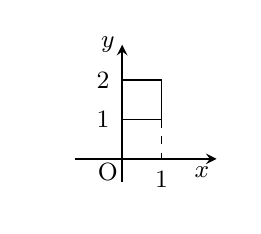
\begin{tikzpicture}[scale=0.5, line width=0.5pt, baseline=(current bounding box.center)]
  \path (-2.4,-1.2) rectangle (2.8,3.0); % 보기 행 사이 여백
  \draw[->, >=stealth, line width=0.7pt] (-1.2,0) -- (2.4,0) node[below left=-1pt, font=\small] {$x$};
  \draw[->, >=stealth, line width=0.7pt] (0,-0.6) -- (0,2.9) node[left=-1pt, font=\small] {$y$};
  \draw[line width=0.6pt] (0,1) rectangle (1,2);
  \draw[dashed, line width=0.4pt] (1,1) -- (1,0);
  \node[below left=-2pt, font=\small] at (0,0) {$\mathrm{O}$};
  \node[below=1pt, font=\small] at (1,0) {$1$};
  \node[left=1pt, font=\small] at (0,1) {$1$};
  \node[left=1pt, font=\small] at (0,2) {$2$};
\end{tikzpicture}
